\documentclass[9pt,twocolumn,twoside]{gsajnl}

\include{hyperref}

\articletype{inv} % article type
% {inv} Investigation 
% {gs} Genomic Selection
% {goi} Genetics of Immunity 
% {gos} Genetics of Sex 
% {mp} Multiparental Populations

\title{Microarray-based detection of genomic signatures related with the tumour recurrence in Glioblastoma patients}

\author[$\ast$,1]{Álvaro Abella-Bascarán}
\author[$\ast$]{Eloi Casals-Puig}
\author[$\ast$]{Samuel Miravet-Verde}

\affil[$\ast$]{Pompeu Fabra University, Barcelona (Spain)}

\keywords{Microarray analysis; tumour recurrence; glioblastoma; temozolomide.}

\runningtitle{GENETICS | INVESTIGATION}

\correspondingauthor{Corresponding Author}

\begin{abstract}

Glioblastomas are notorious for resistance to therapy, and consequently for their frequent recurrence. In order to deal with recurrent tumours more complex treatments are needed, and still the survival is very low. A way to approach this problem would be to have a method to predict which tumours are prone to become recurrent, in order to apply the treatment as soon as possible and give better expectancies to the patients.

In this work, the quality of the data provided by \cite{Murat2008} has been validated, and a different approach has been applied in order to find signatures related to recurrent glioblastoma. The results show that recurrence is far from the consequence of a few altered genes, and it must be seen as the result of a combination of multiple over and underexpressed molecular routes. At the end, we can highlight differences in the expression of genes related to the ability to escape immune response and apoptosis, along with an upregulation of DNA damage repair, cell cycle and division processes, probably favoured by a higher metabolic rate.

\end{abstract}

\setboolean{displaycopyright}{true}

\begin{document}

\maketitle
\thispagestyle{firststyle}
\marginmark
\firstpagefootnote
\correspondingauthoraffiliation{Affiliation correspondence email:  alvaro.abella01@estudiant.upf.edu}

\vspace{-1cm}
\section*{\underline{Introduction}}


%Linkear HTML del supplementary matherial en todo lo que lo diga

Glioblastoma multiforme, involving glial cells, is the most frequent and aggressive brain tumor in humans, with an incidence of 2–3 cases per 100,000 person life-years in Europe and North America \citep{Bleeker2012} and its treatment can involve chemotherapy, radiation and surgery. The median survival presented with standard-of-care radiation and chemotherapy with the alkylating agent temozolomide is only 15 months  \citep{Johnson2012} while the median survival without treatment is 4 and a half months. 

Regretfully glioblastomas are well-known for its resistance to therapy (and consequently for their recurrence). The treatment for this cases requires a more aggressive combination of drugs, including nitrosoureas, temozolomide and bevacizumab, in addition to radiotherapy and surgery \citep{Weller2013}. This approach implies several risks for the patient and, therefore, it is only applied after the relapse of the patient.

Biologically, the resistance to treatment has been initially attributed to DNA-repair proficiency, cell proliferation and, more recently, to the particular biologic behavior of tumor stem-like cells, as it is exposed in the work of Anastasia Murat \citep{Murat2008}. In that case the HOX and EGFR related pathways were identified as the most differentially expressed using clustering techniques and rigid statistical methods. Then, we propose here a more general analysis, to determine the molecular profiles specific for recurrent glioblastoma tumours.

\section*{\underline{Materials and Methods}}

\subsection*{Tumour Samples and Patient Characteristics}

We analyzed data from 80 frozen glioblastoma samples provided by \cite{Murat2008}. The data comprised 70 tumours from initial surgery and 10 samples resected after recurrence. All patients were treated within a phase II or a randomized phase III trial \citep{Stupp2002,Stupp2005}
The study includes 21 females and 55 males, with a median age of 52 (range, 26 to 70 years). Out of the 76 patients, 28 received radiotherapy treatment only, and 48 received TMZ/radiotherapy treatment. 

\subsection*{Gene Expression Profiling}

The microarray data with gene expression profiling was obtained from the Gene Expression Omnibus (GEO) database at \url{http://www.ncbi.nlm.nih.gov/geo/} (accession-number GSE7696). The data had been created from 54675 probes prepared with the Enzo BioArray-High Yield Kit (Enzo Life Sciences, Farmingdale, NY) for double amplification and were hybridized to Affymetrix HG-133Plus2.0 GeneChips (Affymetrix, Santa Clara, CA). The data used had been normalized to the expression of the EIF2C3, DNAJA4, and B2M genes that exhibited little variation in the data set \citep{Murat2008}.

\subsection*{Data Analysis and Statistical Methods}
Analyses were carried out in R, a free software environment available at \url{http://www.r-project.org/}. The full list of packages and modules used can be found in te session information part at the end of the supplementary document. 

\subsubsection*{Work flow and scripts}: in order to ensure the reproducibility of results, all the analysis steps performed can be found in the \href{http://ieoproject.tk/ieo/abella_casals_miravet.html}{supplementary material} in \textit{HTML} format. This file was processed directly from R using 
\href{http://cran.r-project.org/web/packages/knitr/index.html}{knitr} and \href{http://cran.r-project.org/web/packages/markdown/index.html}{markdown}. The file contains detailed explanations about the methodology, statistical interpretation and all the graphics generated during the process. 

\subsubsection*{Quality assessment and Normalization:}
the quality of the microarray data was assessed by a variety of quality checks. Raw chip images were visually inspected to ensure the absence of  artifacts. The intensity distributions of the samples showed a similar poisson distribution, without any artifactual distribution. We used the linear probe level model (PLM) \citep{Bolstad2004, Brettschneider2007} to verify the absence of artifacts in the chip pseudoimages created from the weights and residuals of the sample PLM's. We used Normalized Unscaled Standard Errors (NUSE) \citep{Bolstad2004} to evalute the deviation of the chip probsets, from here, samples with NUSE median value higher than 1.05 were removed. Using the same models, we also evaluated the Relative Log Expression (RLE) values \citep{Bolstad2004, Brettschneider2007} to determine technical biases on particular chips resulting in no particular deviation of the median or the interquartile range found on any sample.

The expression intensities for all probe sets from Affymetrix CEL-files were estimated using robust multiarray average with probe-level quantile normalization followed by median polish summarization \citep{Irizarry2003} as implemented in the BioConductor software (\url{http://www.bioconductor.org/}). The inspection of MA plots (available at \href{http://ieoproject.tk/ieo/abella_casals_miravet.html}{supplementary material}) ensured the absence of fluorescent intensity dependent biases \citep{Bolstad2004}. After the quality assurance process, no samples were discarded from the analysis.

\subsubsection*{Analysis of batch effect and confounding variables:}
the samples were checked for batch effect, first using hierarchical clustering after measuring the Spearman correlation among samples, and then verifying the absence of batch effects by multidimensional scaling. The presence of confounding variables was assessed by means of principal component analysis, and different sources of heterogeneity were analyzed by surrogate variable analysis \citep{Leek2007}. We decided adjust for age and methylation status \citep{Qiu2014} excluding the batch as confounding variable. 

\subsubsection*{Differential Expression}: the list of analyzed probes was reduced using a non-specific filtering \citep{Bourgon2010}, eliminating features with little variation (IQR cutoff = 0.5), consistently low signal across samples, or insufficient annotation. With process we passed from 54675 genes to 10195.

The differential expression analysis of microarray data was done with an empirical Bayes method \citep{Smyth2004} implemented in the Bioconductor package limma. The Benjamini-Hochberg procedure was applied for multiple testing correction (false-discovery rates) \citep{Benjamini1995}. We called Differentially Expressed (DE) genes at 10\% FDR resulting in 255 differentially expressed (DE) genes.

\subsubsection*{Functional Enrichment}: we analysed the enrichment of gene ontology terms (\url{http://www.geneontology.org}) for biological processes (GO BP) using a one-tailed Fisher's exact test \citep{Fisher1922}. The significance of the GO terms is computed conditionally to the significance of its child terms \citep{Alexa2006}. GO terms formed by less than five genes or with less than five DE genes were removed to improve the reliability of the results. This concrete analysis was repeated three times, one considering DE genes in general and two more with only overexpressed and underexpressed genes in the recurrent patients. 

\subsubsection*{Simple GSEA}: Gene Set Enrichment Analysis \citep{Subramanian2005} was carried out using the simple GSEA algorithm \citep{Irizarry2009}, as provided in the \href{http://www.bioconductor.org/packages/release/bioc/html/GSEABase.html}{GSEABase} package from the Bioconductor project. The gene sets used during the analysis are the ones available in the package \href{http://www.bioconductor.org/packages/release/data/experiment/html/GSVAdata.html}{GSVAdata}, with the name `c2BroadSets', once restricted to those which belong to pathways from \href{http://www.genome.jp/kegg/pathway.html}{KEGG}, \href{http://www.reactome.org/}{REACTOME} and \href{http://www.biocarta.com/}{BIOCARTA}. In order to add some robustness to the calculation of the Z-scores, the evaluation was limited to gene sets having 5 or more genes. Finally, only gene sets with an FDR of less than 10\% were called differentially expressed.

\section*{\underline{Results and Discussion}}

The analysis of differential expression showed 255 genes differentially expressed (figure \ref{fig:volcano}) (corrected p-value < 0.1) across the two conditions (recurrent and non-recurrent GBM). From this set of genes we performed a Gene Ontology (GO) enrichment analysis, first using all differentially expressed genes, and after separating by under and overexpression in recurrent tumours. Additionally, a simple GSEA was carried out to check similarities and possible new differentially expressed pathways. The results from this analysis are presented below, including some biological inferences. The GO enrichment analysis are exposed in three different subsections, and the results from the GSEA can be found at the end of the section. A general overview of the results obtained can be found in the table \ref{tab:resume}.

\begin{figure}[!h]
	\centering
	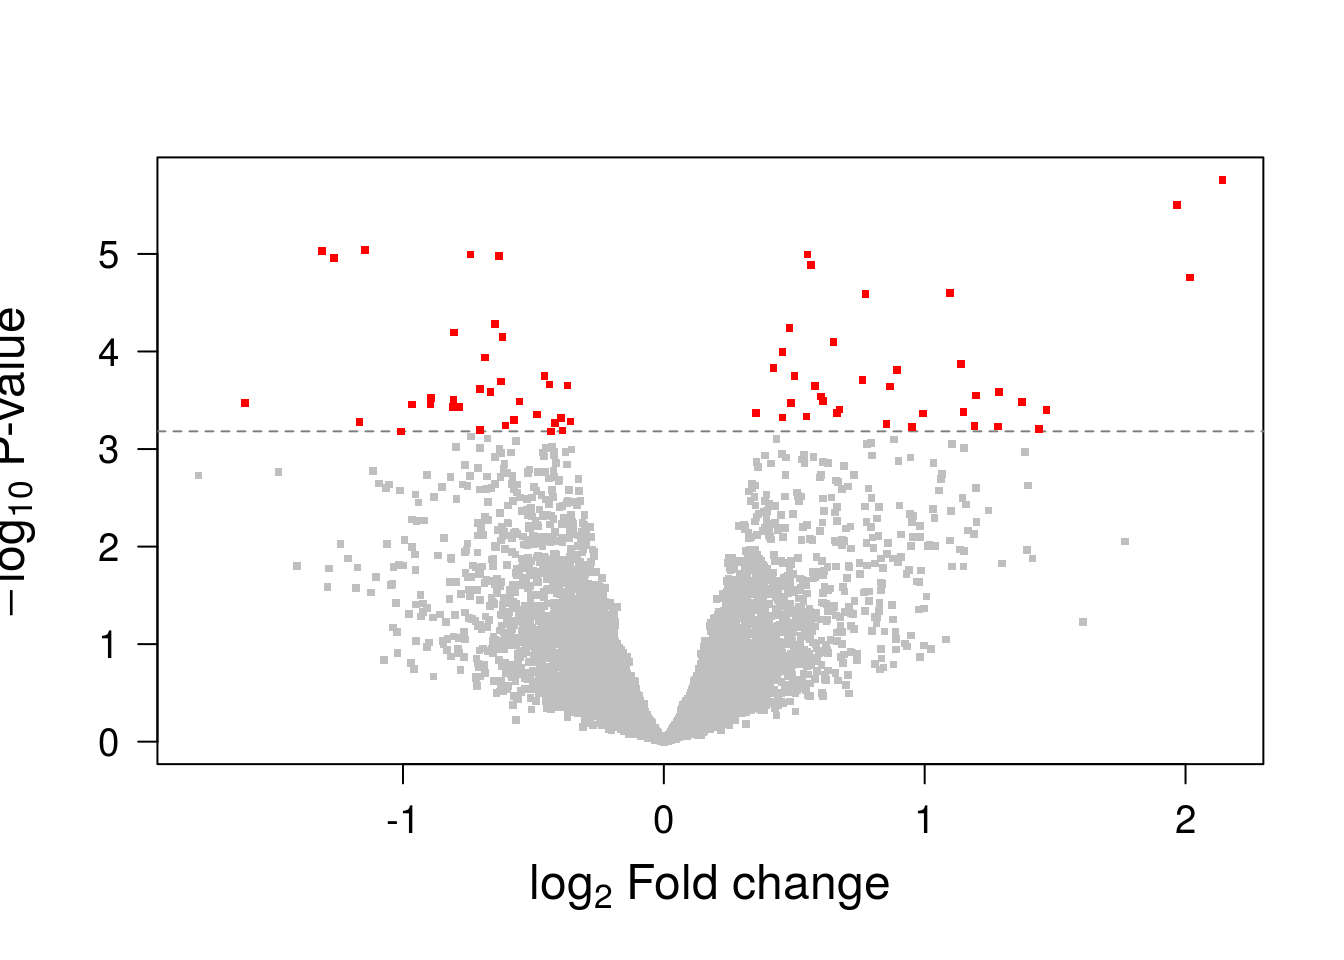
\includegraphics[scale=0.4]{volcano.png}
	\caption{Volcano plot showing DE genes (red), with negative and positive fold changes indicating underexpressed and overexpressed genes, respectively, in recurrent tumours.}
	\label{fig:volcano}
\end{figure}


\begin{table*}[!htbp]
\centering
\caption{\bf Resume of results}
\begin{tableminipage}{\textwidth}
\begin{tabularx}{\textwidth}{m{3.4cm}m{2.6cm}m{1.5cm}m{9.2cm}}
\hline
Condition & Number of terms\footnote{Gene Ontology terms or Pathway terms} & nº genes & Important functions included\\
\hline

General GO Enrichment & 43 & 161 & Metabolic processes, Regulation of differentiation, Immune response, Intracellular transport, Extracellular transport \& Homeostasis, negative regulation of cell cycle G1/S phase transition, Cell adhesion, Anatomical cell structure, Protein modification. \\

Underexpression GO Enrichment & 15 & 66 & Cell surface, Negative regulation of cell cycle, proliferation \& apoptisis, Immune response, Cell adhesion, RNA processing, Negative regulation of protein transport.\\

Overexpression GO Enrichment & 34 & 116 & Negative regulation of cell death \& apoptosis, Metabolic processes, Cell structure organization, Transport and Homeostasis, DNA \& Protein modification, Immune response \& Inflammation.\\

Gene Set Enrichment Analysis & 304 & NA\footnote{No concrete genes were considered as the results come directly from the Expression Set} & Metabolism regulation, Cell cycle regulation, Damage response, Negative regulation of Apoptosis, Immune system. \\

\hline
\end{tabularx}
  \label{tab:resume}
\end{tableminipage}
\end{table*}

\subsubsection*{General Enrichment}: the GO enrichment revealed 43 enriched terms (the corresponding table can found in the supplementary material) when considering together under and overexpressed genes. In total, 161 genes significantly differentially expressed were included in this group.\\
The enrichment include terms related to metabolic processes (eg. glucose metabolic process and hexose biosynthetic process), immune response (eg. regulation of T-cell activation and regulation of lymphocyte proliferation), and cell proliferation (regulation of cell cycle G1/S phase transition and cell proliferation).\\
This profile suggests that glioblastoma recurrence is due to heterogeneous causes, possibly combining a higher ability to escape immune response with an even more dysregulated cell cycle, supported by a higher glucose metabolism.

\subsubsection*{Underexpression Enrichment}: the enrichment with underexpressed DE genes revealed 66 different genes grouped in 15 GO terms (table \ref{tab:under}), among which we can highlight the `apoptotic signaling pathway'. It is known that defects in apoptosis signalling contribute to tumour resistance \citep{Debatin2004}, and we can therefore include it as a feature contributing to recurrence in glioblastoma. This situation of resistance and uncontrolled growth is also favored by the downregulation of pathways negatively related with the proliferation and cell cycle control.\\
In addition, it is interesting to remark the bigger set of genes, 29, present in the `Cell surface receptors pathways'. This could be related with the fact that cancerous cells inhibit the exposure on their surface of cell death receptors, in addition to other possible antigens that could be detected by the immune system \citep{Ozoren2003}.

\subsubsection*{Overexpression Enrichment}: the enrichment done with overexpressed DE genes in recurrent patients revealed 34 different GO terms (table \ref{tab:over}) including a total of 116 different genes. An interesting result is the presence of the enriched terms `exocytosis' and `transport proteins' (both included in the class `Transport and Homeostasis').\\
With respect to exocitosis, it is known that invasion by cancer cells is facilitated by the secretion of enzymes that degrade the extracelular matrix, and that glioma invasion can be inhibited through inhibition of exocytosis \citep{Liu2012}. Recurrence of the tumor could thus be related with a higher capacity to invade new areas.\\
On the other hand, about the `Transport proteins', one of the most common types of cancer resistance consists on the overexpression of drug pumps able to expel the chemotherapeutical drugs from the cell \citep{Borst2012}. The overexpression of proteins with transmembrane transport function could also be related with recurrence, as the tumour cells would be able to avoid the toxic effect of temozolomide by expelling it from the cytosol or just generating gradients in order to avoid the uptake.

\subsubsection*{Gene Set Enrichment Analysis}: with this analysis 304 pathways were found to be differentially expressed in the recurrent tumours. Among all the results, it is interesting to remark the alteration of metabolism, cell cycle, immune system and apoptosis. All of this terms were also present along the gene ontology enrichment analysis.\\
However, this analysis highlights as one of the most important pathways (highest Z-score) the p53-independent DNA damage response from the Reactome database. This result matches with one of the outcomes proposed by Anastasia Murat \citep{Murat2008}, who explains that tumour resistance could be due to a higher ability to repair DNA damages like those produced by temozolomide.\\
In the figure \ref{fig:gsea} six biologically interesting pathways were selected to provide a visual clue of the differential expression among recurrent and not recurrent tumours. For example, in the case of p53-independent repair, it is possibly to see that in recurrent tumours the genes are slightly but consistently overexpressed.\\
The whole list of pathways altered in recurrent tumours can be found in the \href{http://ieoproject.tk/ieo/abella_casals_miravet.html}{supplementary material}.

\begin{figure}[!h]
	\centering
	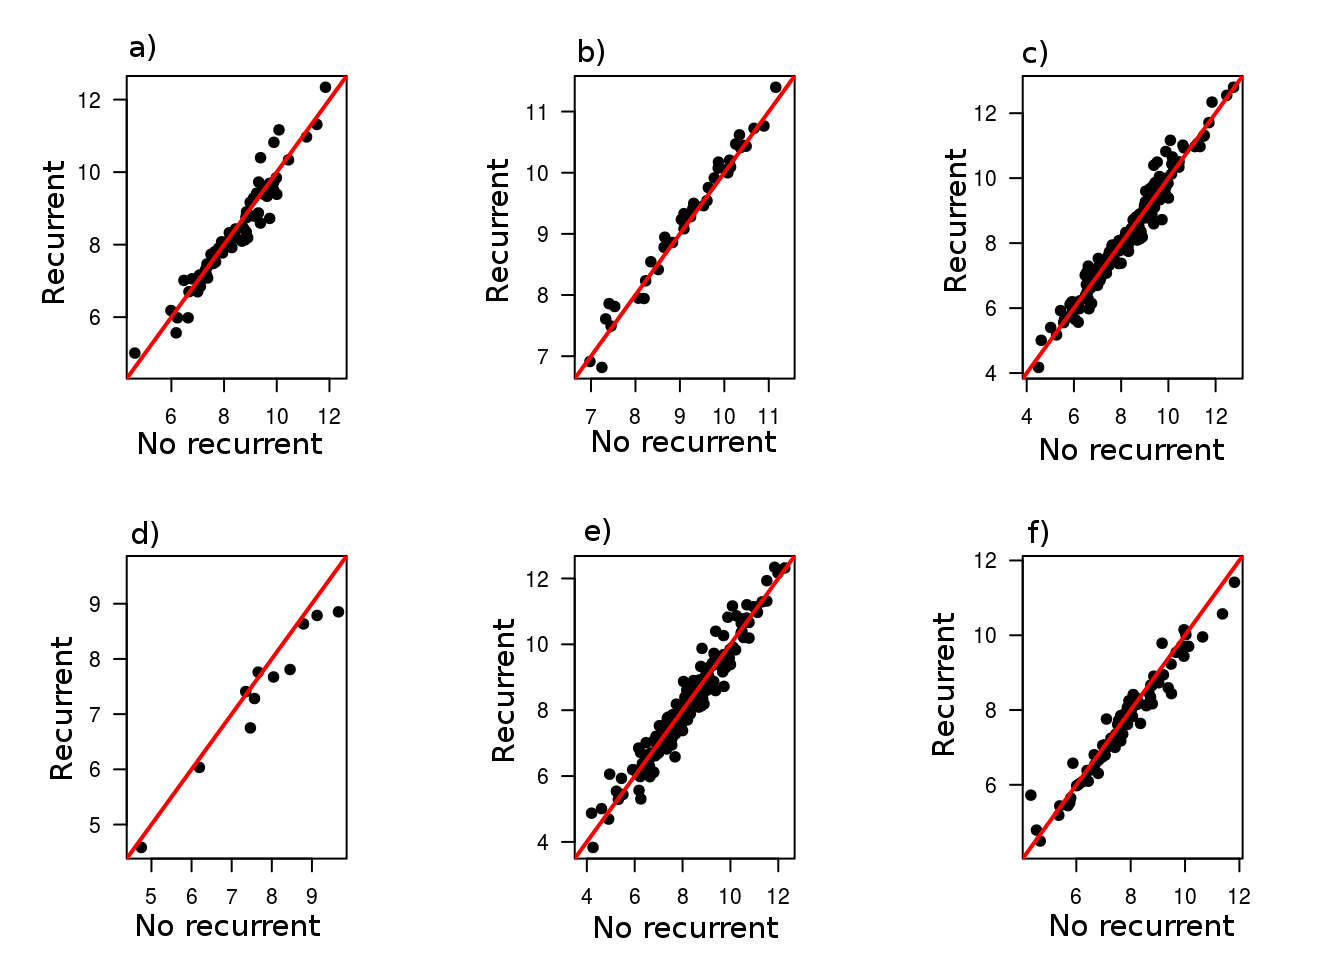
\includegraphics[scale=0.4]{gsea.png}
	\caption{ ALVARO }
	\label{fig:gsea}
\end{figure}

\section*{\underline{Conclusion}}
\cite{Murat2008} show that the genes related with the survival of the patients were those participating in DNA-repair proficiency and stem cell-like behaviour (HOX and EGFR). Here, we have extended their results studying the genetic profile of recurrent patients of glioblastoma. A general overview of the results shows clearly that recurrence cannot be attributed to a single pathway, and it must be seen as the consequence of a multiple set of features, among which we can highlight a higher ability to escape immune response and apoptosis and a more dysregulated cell cycle and monosacharyde metabolism.

As this study is a comparison of recurrent and non-recurrent glioblastoma, we do not dispose of information to know whether this pathways are also enriched in the case of glioblastoma with respect to controls. This information would be useful to draw conclusions on whether recurrence is a consequence of a qualitatively different expression profile, or a quantitative matter (simply the result of a higher expression of cancer-related pathways).

In conclusion, this article exposes a statistically significant genetic profile related with the relapse of glioblastoma patients due to the recurrence of the tumor. As the glioblastoma is one of the most recurrent types of cancer \citep{Bleeker2012}, the definition of a concrete expression profile opens the possibility of having a way to prevent and detect the potential recurrent patients in order to personalize the treatment with the current approaches to recurrent tumours \citep{Weller2013}. 

\bibliography{example-bibliography}

\begin{table*}[htbp]
\centering
\caption{\bf Underexpressed Genes}
\begin{tableminipage}{\textwidth}
\begin{tabularx}{\textwidth}{m{3cm}m{3.5cm}m{1.2cm}m{9.2cm}}
\hline
Biological Processes & GOBPID terms & nº genes & Genes included\footnote{Genes can overlap between GO terms.} \\
\hline

Cell surface receptors pathways & GO:0007166 & 29 & ACTR2, LILRB1, CYLD, ATP6V0E2, EFNB2, CCNY, PEG10, NPB, ADGRD1, TMEM145, IFNGR1, ITGB8, KRAS, NCK1, PDPK1, PRKACB, BIRC6, CEACAM1, RGS18, BMP2, TIAM1, CA2, CPEB4, DYRK2, CBL, KAT2B, ACVR1B, USP34, P2RY14\\

Negative regulation of cell cycle, proliferation \& apoptosis& GO:0051726, GO:0008285, GO:0097190 & 23 & TMOD3, FABP7, LILRB1,TOM1L1, CD33, PRPF40A, DYRK2, NCK1, PRKACB, CYLD, EFNB2, PDPK1, NACC2, ARL6IP5, BIRC6, RBL2, CCNY, TIAM1, SF1, KAT2B, CTBP1, ACVR1B , BMP2\\

Immune response \& Cell Adhesion & GO:0045088, GO:0051249, GO:0002684, GO:0006955, GO:1903037, GO:0034110  & 15 & PDPK1, CYLD, SUSD4, TLR5, CA2, ACTR2, SPPL2A, LST1, HAMP, LILRB1, PRKACB, IFNGR1, ACVR1B, SASH3, NCK\\

Regulation of hydrolase activity & GO:0051336 & 14 & ARL6IP5, CST3, ITSN2, ASAP1, PDPK1, SERPINB6, PRKACB, BIRC6, ARHGAP9, RGS18, BMP2, WNK1, TIAM1, DENND1C\\ 

RNA processing & GO:0006396 & 9 & SRRM1, PAPD4, DHX36, HNRNPA2B1, PRPF40A, RP9, SF1, SLBP, SCAF11\\

Axon Guidance & GO:0007411 & 7 & ACTR2, EFNB2, KIF5C, KRAS, NCK1, TIAM1, ZIC2\\

Negative regulation of protein transport & GO:0051224 & 5 & LYPLA1, LILRB1, CYLD, RHBDF2, DYRK2\\

Activation of protein kinase activity & GO:0032147 & 5 & TOM1L1, KRAS, PDPK1, PRKACB, BMP2\\
\hline
\end{tabularx}
  \label{tab:under}
\end{tableminipage}
\end{table*}

\pagebreak
 

\begin{table*}[htbp]
\centering
\caption{\bf Overexpressed Genes}
\begin{tableminipage}{\textwidth}
\begin{tabularx}{\textwidth}{m{3cm}m{3.5cm}m{1.2cm}m{9.2cm}}
\hline
Biological Processes & GOBPID terms & nº genes & Genes included\footnote{Genes can overlap between GO terms.} \\
\hline

Metabolic Processes & GO:1903050  GO:0042180  GO:0045862  GO:0034655  GO:0005996  GO:0006066  GO:0044265  GO:0043085, GO:0043170 & 82 &  RPP30, ASB1, RTCB, ZNF397, NRBP1, U2AF1, PIGC,  CYR61,  FUCA1, CFH, FBXW7, PCMTD1, PSMD4, CCL5, MAN1B1, PRMT1, MYDGF, COL12A1, SEC31A, PSMC1, DRG1, RPL27A, ATG10, ZNF554, PSMD3, APOL2, TRAPPC2, GSTP1, CYR61,  PMVK, WDR46, FUCA1, CCNB1IP1, BAX, DIS3, STX12, ZNF426, APOL3, SLC35D2, PTGER3, SLC35B4, CTNNB1, RETSAT, RPS9, POLR3GL, RGS4,  FBXW7, SAMD4B, NPY1R, EIF6, USP7, USP7 , INPPL1, TRIP6, PPAP2A,  SEC31A, LIG4, POLR3C, ZCCHC11, ATF5, MFAP4, TOB2, OGT,  PDE10A,TIMM17A, OSR2, ZBTB26, CCS, ZNF791, PIN1, NUDT4, CTSD, DPH5, COPS6, CCL8, RPE65, SNF8, ZNF496,  MAN1B1, OBFC1, APOBEC3F, RPA2\\

Cell structure organization & GO:0043062, GO:0044419, GO:0051234, GO:0051640 & 54 & APOL2, NUDT4, CALU, SLC39A7, CCL8, COL12A1, USP7, EIF6, TMED9, ECM2, BAX, CYR61, ABI3BP, ATG10, CCS, APOL3, SEC31A, ANTXR2, TRAPPC2, CCL5, TRIP6, HNMT, SLC35B4, INPPL1, TIMM17A, TMEM63A, NRBP1, COPS6, PSMC1, SNF8, FBXW7, HOMER3, MCOLN2, STX12, PTGER3, SYTL5, PSMD3, SNCAIP, PSMD4, RPL27A, CTNNB1, CTSD, RPS9, PEX16, RIMS4, WDR46, U2AF1, SLC26A7, ARF5, LIG4, SLC35D2, MFAP4, APOBEC3F\\

Transport and Homeostasis & GO:0006887, GO:0016482, GO:0006816, GO:0072511, GO:0060249,  GO:0051650, GO:0044765 & 40 & SLC35B4, TMEM63A, U2AF1, HOMER3, SLC39A7, MCOLN2, WDR46, OBFC1, SLC26A7, CCS  , TMED9, EIF6, COPA, NRBP1, TIMM17A, APOL2, CALU, SYTL5, NUDT4, SLC35D2, SNCAIP, SNF8, SEC31A, RPL27A, BAX, SYTL5  TIMM17A, STX12, RPS9, CCL5, APOL3, HNMT,  CTNNB1, CCL8, TRAPPC2, TRIP6, RPA2, RPE65, RIMS4, PEX16, PTGER3\\

DNA \& Protein Modification & GO:1903322, GO:0032259, GO:0031400, GO:0006605, GO:0032446, GO:0051338 & 30 & ATG10, SNF8, RPS9, BAX, TIMM17A, PRMT1, PIN1, OGT, PSMD4, FBXW7, PSMC1, HNMT, RPL27A, DPH5, CYR61, GSTP1,  PCMTD1, PSMD3,  CTNNB1, ASB1, PEX16, SEC31A, PIN1, RGS4, MYDGF, TRIP6, HOMER3, CCL5 , WDR46, CCNB1IP1\\

Immune Response \& Inflamation & GO:0002478, GO:0019882, GO:0016032, GO:0001817, GO:0006954  & 27 & CFH, PSMD3, GSTP1, FBXW7, RPS9,  COPS6, PSMC1, POLR3GL,  APOL2, ASB1, SNF8, APOBEC3F, PSMD4, CTSD, BAX, ZCCHC11, RPL27A,  POLR3C, LIG4, PTGER3, APOL3, USP7, PIN1, SEC31A, CTNNB1, CCL8, CCL5\\

Negative regulation of apoptosis \& cell death & GO:0030111, GO:0060548, GO:0043066  & 13 & MYDGF, CYR61, WIF1, CCL5, PSMC1,  ATF5, BAX, PSMD3, CTNNB1, GSTP1, PSMD4, LIG4, ATF5\\

\hline
\end{tabularx}
  \label{tab:over}
\end{tableminipage}
\end{table*}

\end{document}
